\documentclass[12pt]{article}

\usepackage{graphicx}
\usepackage{pgffor}
\usepackage{caption}
\usepackage{subfig}
\usepackage{subcaption}
\usepackage{tabularray}
\usepackage{color}
\usepackage{alltt}
\usepackage{float}
\usepackage{amsmath}
\usepackage{amsthm}
\usepackage{yhmath}
\usepackage{xcolor}
\usepackage{soul}
\usepackage{hyperref}
\usepackage{cleveref}
\usepackage{multirow}
\usepackage{pdfpages}
\usepackage{datetime}


\usepackage{bm}
\usepackage{dsfont}

% blackboard bold 
\newcommand{\ind}{\mathds{1}}
\newcommand{\R}{\mathds{R}}
\newcommand{\N}{\mathds{N}}
\newcommand{\Q}{\mathds{Q}}
\providecommand{\C}{}
\renewcommand{\C}{\mathds{C}}
\providecommand{\P}{}
\renewcommand{\P}{\mathds{P}}
\newcommand{\Z}{\mathds{Z}}
\newcommand{\E}{\mathds{E}}
\newcommand{\K}{\mathds{K}}
\renewcommand{\L}{\mathds{L}}
\newcommand{\V}{\mathds{V}}
\newcommand{\F}{\mathds{F}}
\providecommand{\G}{}
\newcommand{\D}{\mathds{D}}

% bold letters
\newcommand{\bnull}{\bm{0}}
\newcommand{\ba}{\bm{a}}
\newcommand{\bb}{\bm{b}}
\newcommand{\bc}{\bm{c}}
\newcommand{\bd}{\bm{d}}
\newcommand{\be}{\bm{e}}
% \newcommand{\bf}{\bm{f}}
\newcommand{\bg}{\bm{g}}
\newcommand{\bh}{\bm{h}}
\newcommand{\bi}{\bm{i}}
\newcommand{\bj}{\bm{j}}
\newcommand{\bk}{\bm{k}}
\newcommand{\bl}{\bm{l}}
% \newcommand{\bm}{\bm{m}}
\newcommand{\bn}{\bm{n}}
\newcommand{\bo}{\bm{o}}
\newcommand{\bp}{\bm{p}}
\newcommand{\bq}{\bm{q}}
\newcommand{\br}{\bm{r}}
\newcommand{\bs}{\bm{s}}
\newcommand{\bt}{\bm{t}}
\newcommand{\bu}{\bm{u}}
\newcommand{\bv}{\bm{v}}
\newcommand{\bw}{\bm{w}}
\newcommand{\bx}{\bm{x}}
\newcommand{\by}{\bm{y}}
\newcommand{\bz}{\bm{z}}

% bold letters
\newcommand{\bA}{\bm{A}}
\newcommand{\bB}{\bm{B}}
\newcommand{\bC}{\bm{C}}
\newcommand{\bD}{\bm{D}}
\newcommand{\bE}{\bm{E}}
% \newcommand{\bf}{\bm{f}}
\newcommand{\bG}{\bm{G}}
\newcommand{\bH}{\bm{H}}
\newcommand{\bI}{\bm{I}}
\newcommand{\bJ}{\bm{J}}
\newcommand{\bK}{\bm{K}}
\newcommand{\bL}{\bm{L}}
\newcommand{\bM}{\bm{M}}
\newcommand{\bN}{\bm{N}}
\newcommand{\bO}{\bm{O}}
\newcommand{\bP}{\bm{P}}
\newcommand{\bQ}{\bm{Q}}
\newcommand{\bR}{\bm{R}}
\newcommand{\bS}{\bm{S}}
\newcommand{\bT}{\bm{T}}
\newcommand{\bU}{\bm{U}}
\newcommand{\bV}{\bm{V}}
\newcommand{\bW}{\bm{W}}
\newcommand{\bX}{\bm{X}}
\newcommand{\bY}{\bm{Y}}
\newcommand{\hbY}{\hat{\bm{Y}}}
\newcommand{\bZ}{\bm{Z}}


% calligraphic letters
\newcommand{\Acal}{\mathcal{A}}
\newcommand{\Bcal}{\mathcal{B}}
\newcommand{\Ccal}{\mathcal{C}}
\newcommand{\Dcal}{\mathcal{D}}
\newcommand{\Ecal}{\mathcal{E}}
\newcommand{\Fcal}{\mathcal{F}}
\newcommand{\Gcal}{\mathcal{G}}
\newcommand{\Hcal}{\mathcal{H}}
\newcommand{\Ical}{\mathcal{I}}
\newcommand{\Jcal}{\mathcal{J}}
\newcommand{\Kcal}{\mathcal{K}}
\newcommand{\Lcal}{\mathcal{L}}
\newcommand{\Mcal}{\mathcal{M}}
\newcommand{\Ncal}{\mathcal{N}}
\newcommand{\Ocal}{\mathcal{O}}
\newcommand{\Pcal}{\mathcal{P}}
\newcommand{\Qcal}{\mathcal{Q}}
\newcommand{\Rcal}{\mathcal{R}}
\newcommand{\Scal}{\mathcal{S}}
\newcommand{\Tcal}{\mathcal{T}}
\newcommand{\Ucal}{\mathcal{U}}
\newcommand{\Vcal}{\mathcal{V}}
\newcommand{\Wcal}{\mathcal{W}}
\newcommand{\Xcal}{\mathcal{X}}
\newcommand{\Ycal}{\mathcal{Y}}
\newcommand{\Zcal}{\mathcal{Z}}

% greek letters
\newcommand{\eps}{\varepsilon}
\newcommand{\sd}{\sigma}
\newcommand{\ssd}{\sigma^2}
\newcommand{\gb}[1]{\beta_#1}
\newcommand{\hbe}[1]{\hat{\beta}_#1}
\newcommand{\beps}{\bm{\varepsilon}}
\newcommand{\hbeps}{\hat{\bm{\varepsilon}}}
\newcommand{\balpha}{\bm{\alpha}}
\newcommand{\bbeta}{\bm{\beta}}
\newcommand{\hbbeta}{\hat{\bm{\beta}}}
\newcommand{\bchi}{\bm{\chi}}
\newcommand{\bdelta}{\bm{\delta}}
\newcommand{\bepsilon}{\bm{\epsilon}}
\newcommand{\bphi}{\bm{\phi}}
\newcommand{\bgamma}{\bm{\gamma}}
\newcommand{\betah}{\bm{\etah}}
\newcommand{\btheta}{\bm{\theta}}
\newcommand{\htheta}{\hat{\theta}}
\newcommand{\hbtheta}{\hat{\bm{\theta}}}
\newcommand{\vtheta}{\vartheta}
\newcommand{\bvtheta}{\bm{\vartheta}}
\newcommand{\hbvtheta}{\hat{\bm{\vartheta}}}
\newcommand{\hTheta}{\hat{\Theta}}
\newcommand{\btau}{\bm{\tau}}
\newcommand{\htau}{\hat{\tau}}
\newcommand{\hbtau}{\hat{\bm{\tau}}}
\newcommand{\biota}{\bm{\iota}}
\newcommand{\bkappa}{\bm{\kappa}}
\newcommand{\blambda}{\bm{\lambda}}
\newcommand{\bmu}{\bm{\mu}}
\newcommand{\bnu}{\bm{\nu}}
\newcommand{\bomikron}{\bm{\omikron}}
\newcommand{\bpi}{\bm{\pi}}
\newcommand{\hbpi}{\hat{\bm{\pi}}}
\newcommand{\bxi}{\bm{\xi}}
\newcommand{\bzeta}{\bm{\zeta}}
\newcommand{\bomega}{\bm{\omega}}
% logic
\newcommand{\equivto}{\Leftrightarrow}
\newcommand{\quequiv}{\quad \equivto \quad}
\newcommand{\impl}{\Rightarrow}
\newcommand{\quimpl}{\quad \Rightarrow \quad}
\newcommand{\implby}{\Leftarrow}

% linear algebra
\newcommand{\tr}{\operatorname{tr}}
\newcommand{\spann}{\operatorname{span}}
\newcommand{\col}{\operatorname{col}}
\newcommand{\rang}{\operatorname{rang}}
\newcommand{\diag}{\operatorname{diag}}
\renewcommand{\vec}{\operatorname{vec}}
\newenvironment{roweqmat}[1]{\left(\array{@{}#1@{}}}{\endarray\right)}

\newcommand{\la}{\langle}
\newcommand{\ra}{\rangle}
\newcommand{\inner}[1]{\langle #1 \rangle}
\newcommand{\proj}{\operatorname{proj}}


\renewcommand{\bar}{\overline}

% statistics
\providecommand{\Pr}{}
\renewcommand{\Pr}{\mathbb{P}}
\newcommand{\var}{{\mathds{V}\mathrm{ar}}}
\newcommand{\bias}{{\operatorname{bias}}}
\newcommand{\abias}{{\mathrm{ABias}}}
\newcommand{\AMSE}{{\mathrm{AMSE}}}
\newcommand{\AMISE}{{\mathrm{AMISE}}}
\newcommand{\cov}{{\mathds{C}\mathrm{ov}}}
\newcommand{\corr}{{\mathrm{Corr}}}
\newcommand{\ov}{\overline}
\newcommand{\wh}[1]{\widehat{#1}}
\newcommand{\wt}[1]{\widetilde{#1}}
\newcommand{\tod}{\stackrel{d}{\to}}
\newcommand{\Cov}{\text{Cov}}

\newcommand{\sumin}{\sum_{i = 1}^n}
\newcommand{\sumjn}{\sum_{j = 1}^n}


\newcommand{\KL}{\operatorname{KL}}
\DeclareMathOperator*{\argmin}{arg\,min}
\DeclareMathOperator*{\argmax}{arg\,max}


\newcommand{\softmax}{\operatorname{SoftMax}}
\newcommand{\layernorm}{\operatorname{LayerNorm}}
\newcommand{\avg}{\operatorname{avg}}
\newcommand{\relu}{\operatorname{ReLu}}

% figure environment with scaling in multiples of \textwidth
\newcommand{\fig}[1][1]{
  \includegraphics[width = #1\textwidth]
}

% footnote without mark
\makeatletter
\def\blfootnote{\gdef\@thefnmark{}\@footnotetext}
\makeatother

\newcommand{\envbreak}{ \, \\[-12pt]}
\newcommand{\tw}{\textwidth}


% Sonstiges
%\newcommand*\bigcdot{\mathpalette\bigcdot@{.5}}
%\newcommand*\bigcdot@[2]{\mathbin{\vcenter{\hbox{\scalebox{#2}{$\m@th#1\bullet$}}}}}
\newcommand{\hr}{\centerline{\rule{3.5in}{1pt}}}

\definecolor{mycolor}{HTML}{3C8031}
\newcommand{\tc}[1]{\textcolor{red}{#1}}

\usepackage{longtable}
\usepackage{booktabs}

\newcommand{\minimage}[2]{%
  \includegraphics[width=0.08\textwidth]{../figs/cifar_images_examples/#1_#2.png}%
}

\newcommand{\minimagerow}[1]{
  \minimage{#1}{0} & \minimage{#1}{1} & \minimage{#1}{2} & \minimage{#1}{3} & \minimage{#1}{4} & \minimage{#1}{5} & \minimage{#1}{6} & \minimage{#1}{7} & \minimage{#1}{8} & \minimage{#1}{9}    
}

\newcommand*{\vertbar}{\rule[-1ex]{0.5pt}{2.5ex}}
\newcommand*{\horzbar}{\rule[.5ex]{2.5ex}{0.5pt}}


\newcommand{\mytitle}{FairML and the SQF dataset}
\newcommand{\myname}{\large Juliet Fleischer}
\newcommand{\mysupervisor}{Dr. Ludwig Bothmann}

\newcommand{\thesuffix}[1]{%
  \ifnum#1=1 st%
  \else\ifnum#1=2 nd%
  \else\ifnum#1=3 rd%
  \else th%
  \fi\fi\fi}

% Manually define the date format with the ordinal suffix
\newcommand{\mydate}{%
  ~\ifcase\month\or
  January\or February\or March\or April\or May\or June\or July\or August\or
  September\or October\or November\or December\fi, \the\day\thesuffix{\day} \number\year}

\usepackage[a4paper, width = 160mm, top = 35mm, bottom = 30mm, 
bindingoffset = 0mm]{geometry}
\usepackage[utf8]{inputenc}
\usepackage{ragged2e}
\usepackage{xcolor}
% \usepackage[round, comma]{natbib}
\usepackage[backend=biber, style=authoryear]{biblatex}
\addbibresource{../literature.bib}
\usepackage{fancyhdr}
\newcommand{\changefont}{%
    \fontsize{8}{11}\selectfont
}
\hypersetup{
  colorlinks = true,
  linkcolor = black,
  urlcolor = black,
  citecolor = black}
\pagestyle{fancy}
\fancyhead{}
\fancyhead[R]{\changefont{\mytitle}}
\fancyfoot{}
\fancyfoot[R]{\thepage}
\setlength{\headheight}{14.5pt}
\setlength{\parindent}{0pt}
\interfootnotelinepenalty = 10000

% ------------------------------------------------------------------------------
% MAIN -------------------------------------------------------------------------
% ------------------------------------------------------------------------------
\IfFileExists{upquote.sty}{\usepackage{upquote}}{}
\begin{document}

% FRONT PAGE -------------------------------------------------------------------
 
\begin{titlepage}
\begin{center}
    
\LARGE
Seminar Thesis

\vspace{0.5cm}
      
\rule{\textwidth}{1.5pt}
\LARGE
\textbf{\mytitle}
\rule{\textwidth}{1.5pt}
   
\vspace{0.5cm}
      
\large
Department of Statistics \\
Ludwig-Maximilians-Universität München

\vfill

\Large
\textbf{\myname}

\vfill

\large

Munich, \mydate
      
\vfill


\includegraphics[width = 0.4\textwidth]{../figures/sigillum.png}

\vfill

\normalsize
Submitted in fulfillment of the requirements for the degree of B. Sc.
\\
Supervised by \mytitle

\end{center}
\end{titlepage}

% CONTENTS ---------------------------------------------------------------------

\pagenumbering{Roman}
\newpage
\begin{abstract}

In the first half of this paper we provide an introduction to the most common metrics and methods in fair machine learning. We then apply the theoretical concepts to the New York Stop, Question and Frisk dataset, which will showcase difficulties that come with fairness in practice. This leads us to explore the problem of selection bias and related issues. We turn our focus to studies that have worked with the SQF dataset and established interesting theoretical results; residual unfairness, bias reversal and bias inheritance.
Value of this paper: compare and contrast traditional fairness metrics, use them in a real world setting, show its limitations in this setting, present how they are adressed in more advanced ways and try to explain why traditional metrics can not reflect the whole situation.

\end{abstract}


\newpage
\tableofcontents
\newpage


% CHAPTERS ---------------------------------------------------------------------

\pagenumbering{arabic}
    
\section{Introduction}
% \label{intro}
% As algorithms are increasingly used to make decisions that affect people's lives, it is important to ensure that these decisions are fair. 
... the field of fiar machine learning. Interesting findings, recent developments, dynamic field.
limitations: unclear definitions, same datasets used over and over again.
This paper is an uncommon introduction to fairness. In "chapter ..." it provides the reader with the most common fairness metrics and methods, found in other introductions
but then in "Chapter ...." we apply them more uncommon dataset. SQF.
Since x the police in NYC is allowed to stop individuals if they have ...
Our case study will showcase difficulties that come with fairness in practice. This leads us to explore other studies that have worked with SQF data in "chapter ...". 

\section{Related Work}
\section{Fairness Metrics}
% \section*{Definitions of Fairness in Machine Learning}
When one starts to get into the topic of fairness in machine learning, it is easy to get overwhelmed by the sheer amount of definitions and metrics that are out there. In this chapter we try to group them in an intuitive way and motivate them in the hope to bring some clarity to readers. It is helpful to group fairness metrics in the following ways.
\begin{enumerate}
    \item Group fairness vs. individual fairness
    \item observational vs. causality-based criteria
\end{enumerate}

Broadly speaking, group fairness aims to create equality between groups and individual fairness aims to create equality between two individuals within a group. Observational fairness metrics act descriptive and use the observed distribution of random variables characterizing the population of interest to assess fairness while causality-based criteria make assumptions about the causal structure of the data and base their notion of fairness on this.
On the basis of these fundamental ideas, a plethora of formalizations have emerged. Most of them concern themselves with defining fairness for a binary classification task and one binary protected attribute (PA).
The extension to a multiclass PA is the easiest. The extension to multiple sensitive attributes, on the other hand, brings challenges with it. Also, the extension from binary classification to other tasks, such as neural networks, LLMs and other models is subject of ongoing research. As this work is meant to help you start thinking about fairness in machine learning, we will limit ourselves to the binary classification case.
To bring more clarity we will illustrate the general fairness metrics already in the context of the SQF dataset.

\subsection{Group fairness}
\begin{table}
    \begin{tabular}{lll}
        \toprule
        Independence & Separation & {Sufficiency} \\
        \midrule
        $\hat{Y} \perp A$ & $\hat{Y} \perp A | Y$ & {$Y \perp A | \hat{Y}$}\\
        \bottomrule
    \end{tabular}
\end{table}

The notion of fairness underlying group metrics is that discrimination of certain groups of the population defined via the PA should be prevented. The groups metrics presented here are observational metrics. They can be separated into three main categories, independence, separation, and sufficiency. 

\subsubsection*{Independence}
Independence is in a sense the simplest group fairness metric. It requires that the prediction $\hat{Y}$ is independent of the protected attribute $A$, so $\hat{Y} \perp A$. This is fulfilled when for each group the same proportion is classified as positive by the algorithm. In other words, the positive prediction ratio (ppr) should be the same for all values of $A$. For a binary classification task with binary sensitive attribute this can be formalized as \\
\textbf{demographic parity/statistical parity}
$$P(\hat{Y} | A = a) = P(\hat{Y} | A = b)$$
This indeed seems like a simple, perhaps too simple definition of fairness, as it only looks the distribution of $\hat{Y}$ conditioned on the group membership. There are extensions of this idea, such as conditional statistical parity. This metric allows to condition on A and a set of legitimate features E. For instance, predictive parity would mean that we require equal prediction ratios between PoC and white people while conditional statistical parity requires equal prediction ratios between PoC and white people who \textit{live within the same borough of New York} (E = borough). This can be seen as a more nuanced approach, as it allows tacking additional information into account.
The other two groups of group fairness metrics, Separation and Sufficiency can both be derived from the error matrix.
\begin{center}
    \renewcommand{\arraystretch}{1.5}  % Increase row height for a more square-like appearance
    \begin{tabular}{c|c|c|}
        \hline
        & \(Y = 0\) & \(Y = 1\) \\
        \hline
        \(\hat{Y} = 0\) & TN & FN \\
        \hline
        \(\hat{Y} = 1\) & FP & TP \\
    \end{tabular}
\end{center}

\subsubsection*{Separation}
Separation requires independence between $\hat{Y}$ and $A$ conditioned on the true label $Y$, so $\hat{Y} \perp A | Y$. This means that the focus is on equal error rates between groups, which gives rise to the following list of fairness metrics:
\begin{itemize}
    \item Equal opportunity/ False negative error rate balance $$P(\hat{Y} = 0 | Y = 1, A = a) = P(\hat{Y} = 0 | Y = 1, A = b)$$ or $P(\hat{Y} = 1 | Y = 1, A = a) = P(\hat{Y} = 1 | Y = 1, A = b)$
    \item Predictive equality/ False positive error rate balance $$P(\hat{Y} = 1 | Y = 0, A = a) = P(\hat{Y} = 1 | Y = 0, A = b)$$ or \\ $P(\hat{Y} = 0 | Y = 0, A = a) = P(\hat{Y} = 0 | Y = 0, A = b)$ 
    \item Equalized odds $$P(\hat{Y} = 1 | Y = y, A = a) = P(\hat{Y} = 1 | Y = y, A = b) \forall y \in \{0, 1\}$$ 
    \item Overall accuracy equality: $$P(\hat{Y} = Y | A = a) = P(\hat{Y} = Y | A = b)$$ 
    \item Treatment equality: $$\frac{\text{FN}}{\text{FP}} \big|_{A = a} = \frac{\text{FN}}{\text{FP}} \big|_{A = b}$$
\end{itemize}

Equal opportunity requires the false negative rates, the ratio of actual positive people that were wrongly predicted as negative, to be equal between groups.
Therefore, it is also called false negative error rate balance. When there false negative rates are equal between groups, then the true positive rates between groups are also equal.
This means requiring equal false negative rates or equal true positive rates between groups results in the same effect. Predictive equality follows the same principle as equal opportunity but instead of focusing on the false negatives, it focuses on the false positives. Again, if a classifier has equal false positive rates between groups, it also has equal true negative rates.
Equalized odds combines equal opportunity and predictive equality. It requires that the false positive and true positive rates are equal between groups, and is in this sense stricter than either of them alone. \\
In itself, these error rates are detached from the context of fairness and used in general in machine learning to assess the performance of a classifier. In essence the group metrics we outlined so far do nothing other than picking a performance metrics from the confusion matrix and requiring it to be equal between two (or more) groups in the population.
This means the well-known trade-offs for example between false positive and true positive rate are also present in the fairness metrics. As more people get correctly classified as positive usually also more people get wrongly classified as positive. {\color{red}Source}
With this comes the difficulty to choose "the right" metric for the specific task. In general one can think about this in the same way as when choosing a performance metric for a binary classifier.
In setting in which a positive prediction leads to a harmful outcome, as in the SQF setting, it often makes sense to focus on minimizing the false positive rate, while a higher false negative rate is accepted as a trade-off.
This argumentation follows the idea of. The authors distinguish between punitive and assistive tasks to help choose the right fairness metric. For punitive tasks metrics that focus on false positives, such as predictive equality are more relevant. For assistive tasks, such as deciding who receives some kind of welfare, a focus on minimizing the false negative rate could be more relevant, so equal opportunity would be more suitable.

\subsubsection*{Sufficiency}
Sufficiency requires independence between $Y$ and $A$ conditioned on $\hat{Y}$, so $Y \perp A | \hat{Y}$. Intuitively this means that we want a prediction to be equally credible between groups. When a white person gets a positive prediction the probability that it is correct should be they same as for a black person. This leads to the following fairness metrics:
\begin{itemize}
    \item Predictive parity/ outcome test requires that the probability of actually being positive, given a positive prediction is the same between groups. $$P(Y = 1 | \hat{Y} = 1, A = a) = P(Y = 1 | \hat{Y} = 1, A = b)$$
    \item Equal true negative rate follows the same principle as predictive parity. It requires that the probability of actually being negative, given a negative prediction is the same between groups.: $$P(Y = 0 | \hat{Y} = 0, A = a) = P(Y = 0 | \hat{Y} = 0, A = b)$$
    \item If we instead look at errors again, we can require equal false omission rates: $$P(Y = 1 | \hat{Y} = 0, A = a) = P(Y = 1 | \hat{Y} = 0, A = b)$$
    \item Or equal false discovery rate: $$P(Y = 0 | \hat{Y} = 1, A = a) = P(Y = 0 | \hat{Y} = 1, A = b)$$ 
    \item Conditional use accuracy equality: $$P(Y = 1 | \hat{Y} = 1, A = a) = P(Y = 1 | \hat{Y} = 1, A = b) \land P(Y = 0 | \hat{Y} = 0, A = a) = P(Y = 0 | \hat{Y} = 0, A = b)$$
\end{itemize}

False omission describes the case in which an actual positive person is predicted as negative and can be highly relevant in assistive settings, such as description of a medical treatment. False discovery rate describes the case in which an actual negative person is predicted as positive. This should be taken into account in punitive settings, in which we do not want to convict innocent people.
Just as for equalized odds as Separation metric, we can build a stronger Sufficiency metric requiring multiple conditions to hold simultaneously, e.g. conditional use accuracy equality.
Hopefully, the pattern becomes clear now. While it is easy to get overwhelmed by the amount of definitions at first, taking a closer look, it becomes clear that they are constructed in a structured way. In fact, equal false omission rate and equal false discovery rate were not introduced in the paper \cite{verma2018} but are implemented in \texttt{mlr3fairness}, and it is clear that they follow the same pattern as the other metrics.

Most (binary) classifiers work with predictions scores and a hard label classifier is applied only afterwards in form of a threshold criterion. It should therefore come as no surprise that instead of formulating fairness with $\hat{Y}$ there exist fairness metrics that use the score $S$, which typically represents the probability of belonging to the positive class. Instead of conditioning on $\hat{Y}$ as Separation metrics, we can simply condition on $S$ and define: \\
Calibration: $$P(Y = 1 | S = s, A = a) = P(Y = 1 | S = s, A = b)$$
Calibration requires that the probability for actually being positive, given a score $s$ is the same between groups. So the idea is a more fine-grained version of predictive parity. As the score can usually take values from the whole real number line, this can in practice be implemented by binning the scores \cite{verma2018}.

To compare the group fairness criteria, sufficiency takes the perspective of the decision-making instance, as usually only the prediction is known to them in the moment of decision. For example, the police, who do not yet know the true label at the time when they are supposed to decide whether someone would become a criminal.
As separation criteria condition on the true label Y it is suitable when we can be sure that $Y$ is free from any bias, so to say when $Y$ was generated via an objectively true process (this will become clearer in the chapter on bias).
Independence is best, when we want to enforce a form of equality between groups, regardless of context or any potential personal merit. While this seems to be useful in cases in which the data contains complex bias, it is unclear whether these enforcements have the intended benefits, especially over the long term. {\color{red}{Reference?}}.
It is good to understand the difference in perspectives each of the group fairness metrics take, because many of them cannot be satisfied simultaneously. This is known as the impossibility theorem \cite{hardt2016}. This means one has to decide on either Independence, Separation or Sufficiency and the choice should fit the context of the data and the decision-making process. Lastly, we note that these are not all the group fairness metrics that exist, but broadly speaking other metrics are variations of the presented ones. Some more metrics are listed in the appendix.

\subsection{Individual fairness}
If we want to equalize e.g. the false positive rates between two groups and currently group a has a higher false positive rate than group b, this would lead us to lowering the prediction threshold for b, such that more actual negative people would get classified as positive. Or if we would need to set a higher threshold for group a, such that it becomes harder for them to be classified as positive. Depending on the context, either option can seem unfair. So by trying to equalize a given metric between groups, it can happen that individuals within a group are treated unequally. Individual metrics therefore shift the focus. The underlying idea of fairness is that similar individuals should be treated similarly.
\subsubsection*{Fairness through awareness (FTA)}
FTA formalizes this idea as Lipschitz criterion. $$d_Y(\hat{y_i}, \hat{y_j}) \leq \lambda {d_X}(x_i, x_j)$$
$d_Y$ is a distance metric in the prediction space, $d_X$ is a distance metric in the feature space and $\lambda$ is a constant.
The criterion puts an upper bound to the distance between predictions of two individuals, which depends on the features of them. In other words, if two people are close in the feature space, they also should be close in the prediction space. The challenge of FTA is the definition of the equality in the feature space. \cite{castelnovo2022} states "defining when two individuals are similar is not much different from defining fairness in the first place".
In the SQF context, it could make sense to define similar individuals based on yearly income, age and neighbourhood.
Yet one could easily argue that taking the criminal history into account is important as well. After the decision for a legitimate set of features has been made, the next challenge is to choose a distance metric that appropriately captures the conceptual definition of similarity defined via the selected features.
FTA does not have one clear solution and requires domain knowledge and the choice of $d_X$ should take context-specific information into account.

\subsection*{Fairness through unawareness (FTU) or blinding}
In contrast to FTA, blinding should give a simple, context-independent rule. It tells us to not use the protected attribute explicitly in the decision-making process. When training a classifier this means discarding the PA during training.
Since FTU is a more procedural rule than a mathematical definition, there exist multiple ways to test whether the blinding worked for a classifier. One approach is to simulate a doppelgänger for each observation in the dataset. This doppelgänger has the exact same features except the protected attribute, which is flipped.
If both these instances have the same prediction, the algorithm would satisfy FTU \cite{verma2018}. \footnote{This can be seen as a from of FTA, in which we chose the distance metric to measure a distance of zero only if two people are the same on all their features except for the protected attribute. In this special case FTA and FTU are measured in the same way.} Other ways to assess FTU can be found in \cite{verma2018}. 
A problem blinding has been proxies. These are variables that are strongly correlated with the sensitive attribute. It is not enough to simply mask the information of the sensitive attribute during training because discrimination can persist via these proxies.
For SQF this would mean that we remove the race attribute during training.
A person's ethnicity, however, is strongly correlated with their place of residence. Thus, indirect discrimination based on ethnicity remains, even though the information was not directly available during training. \textbf{Suppression} extends the idea of blinding and the goal is to develop a model that is blind to not only the sensitive attribute but also the proxies. The drawback is, that it is unclear when a feature is sufficiently high correlated with the sensitive attribute to be counted as proxy. Additionally, we could lose important information by removing too many features \cite{castelnovo2022}.

\subsection{Causality-based fairness metrics}
In contrast to observational fairness metrics, causality-based notions ask whether the sensitive attribute was the \textit{reason} for the decision. If a certain (harmful) decision was made \textit{because of} the value of the sensitive attribute of a person, we deem the algorithm as unfair.
% There are causality-based concepts that focus on group-level fairness and also some that focus on individual-level fairness. We want to give an intoduction to all of them, but since this category requires a new theory we will not get into great detail.

\textbf{Group-level}: FACE, FACT (on average or on conditional average level) \parencite{Zafar2017PPNFC}\\
\textbf{Individual-level}: counterfactual fairness, path-based fairness \parencite{kusner} 
The two most common individual fairness metrics are counterfactual fairness and path-based fairness.


\subsection{Comparison and Summary}

The difference between observational and causal clear, really different approach. The division in group and individual fairness metric actually more of a nuanced differentiation. The observational metrics can rather be ordered on a plane, depending on how much information of the situation via other features X they allow.
Traditional group metrics like demographic parity, equal error rate metrics and sufficiency metrics only work with the distribution of $Y, \hat{Y}, X, A$. The individual fairness metrics take more information of the non-sensitive feature into account in order to define similarity. Metrics such as conditional demographic parity lie in between, as we allow for a relevant subset of non. Sensitive feature to be part of the definition.
\cite{castelnovo2022} therefore depict this as a plane.
The amount of approaches to measure fairness shows the complexity of the topic. There is not \textit{the} right fairness metric to choose, but there can be the best one depending on the context and the data. The next section will present ways to digitate algorithmic bias once detected by one of the fairness metrics.



\section{Fairness Methods}
\subsection{Fairness methods}
Another question fair machine learning deals with is how algorithms can be adjusted so that they fulfil one of the above fairness metrics.
Depending on when they take place in the machine learning pipeline, we distinguish between
\begin{enumerate}
    \item Pre-processing methods
    \item In-processing methods
    \item Post-processing methods
\end{enumerate}
Pre-processing methods follow the idea that the data should be modified before training, so that the algorithm learns on "corrected" data. Reweighing observations before training is an example for a preprocessing method. The idea is to assign different weights to the observations based on relative frequencies, so that the algorithm learns on a balanced dataset \cite{caton2024}.\\
In-Processing methods modify the optimization criterion, such that it also accounts for a chosen fairness metric. Introducing a regularization term to the loss function is one example of such modifications.\\
Post-processing methods work with black box algorithms, just like preprocessing methods. We only need the predictions from the model to adjust them so that again a chosen fairness metric is fulfilled. One example for this is thresholding, where we set group specific thresholds to re-classify the data after training (\cite{hardt2016}).
Depending on the task (regression, classification) and the model there are highly specified and advanced methods. For the case study in chapter 3, we limit ourselves to methods from the \texttt{mlr3fairness} package.
% mlr3fairness currently has two preprocessing methods, one postprocessing method and several fairness adjusted models implemented. We decide to use a reweighing methods that works with assigning weights to the observations to equalise the distribution of $P(Y|PA)$.
% The inprocessing method is a fairness-adjusted logistic regression implemented in mlr3fairness inspired by Zafar et. al. This method optimises for statistical parity (independence). The postprocessing method we choose aims for equalised odds and it works by randomly flipping a subset of predictions with pre-computed probabilities in order to satisfy equalised odds constraints.

\subsection{Bias and the feedback loop}
Before the application on real data, to introduce different types of biases and the context in which the ADM is embedded.
Used to assist decision-making, the machine learning model influences if someone gets admitted to college, receives a loan or is released from prison.
The circumstances of a decision are made measurable by collecting data. The algorithm learns from this data to make an optimal prediction, on which the decision-makers base their judgement on. This decision will shape the reality, which reflects in new data. This means the algorithm does not exist in isolation, but depends on the data and shapes the user's actions.\\ 
\cite{mehrabi2022} call this the data, algorithm, and user interaction feedback loop. At each stage, bias can be introduced into the process. More dangerous, bias can even be amplified as the algorithm influences decision-making on a large scale.
Consequently, every fairness project comes with the responsibility to understand the data-generating process and gain clarity on how the algorithm will be deployed in the real-world.\\
The data, algorithm, and user interaction feedback loop also helps in distinguish between various types of bias. \autoref{fig:bias_loop} depicts one exemplary type of bias for each stage of the feedback loop. It can be crucial to think about which type of bias might be relevant in a given situation as this should influence the definition of fairness and the choice of fairness adjustments. This will also become evident as we examine the SQF dataset.

\begin{figure}
    \centering
    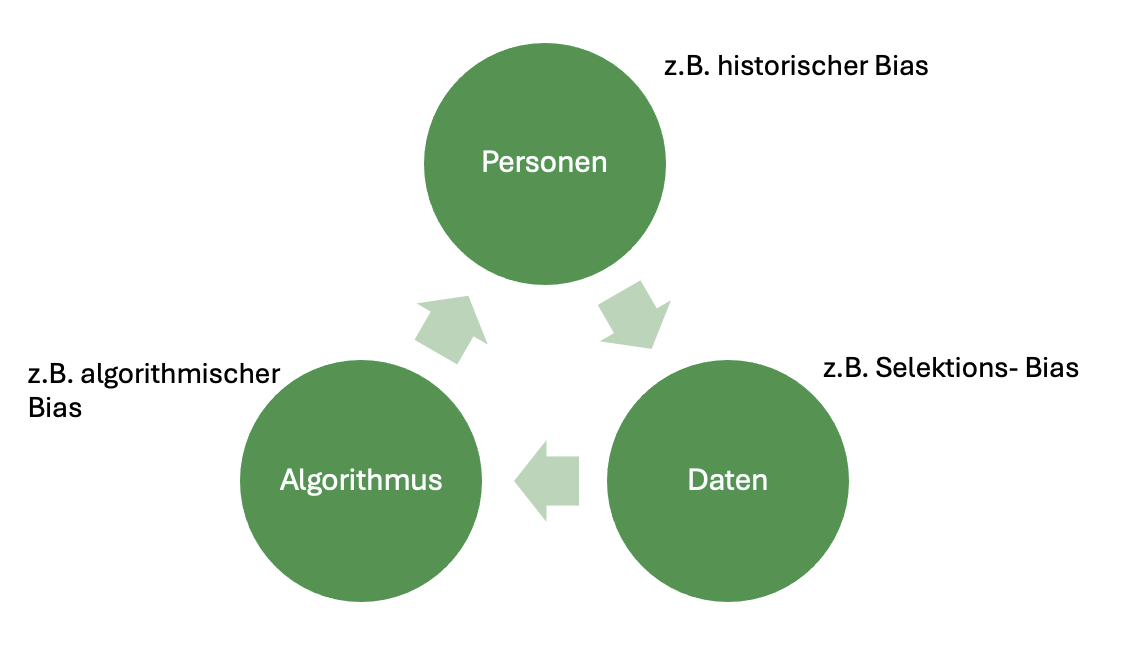
\includegraphics[width=0.7\textwidth]{../figures/bias_loop.png}
    \caption{The bias loop.}
    \label{fig:bias_loop}
\end{figure}

% \subsection*{Bias}
% We want to end this general introduction into fair machine learning by outlining the context in which the algorithm is usually embedded. On this note we also advice practitioners to think about the source of bias that could be present in your situation, as this \textit{should} influence how fairness is defined and what fairness adjustments are appropriate. This will motivate the potential difficulties that can arise when implementing fairness in the real world.
% \cite{caton2024} describe the situation as follows. The algorithm is embedded in a feedback loop with the user and data.
% We as a society make decision, which reflect our reality. We make our reality measurable by collecting data. The algorithm learns from this data and makes predictions, on which we base new decisions. 
% At each of these three points bias can be introduced into the process and, above all, bias can also be reinforced in the course of this process.
% In the context of the Stop, Question, and Frisk data, historical bias and selection bias are probably the most relevant sources of bias.
% Historical bias can shows itself in different ways. In our case it would mean that we assume that some people in our data have repeatedly experienced discrimination in terms of being arrested.
% Selection bias refers to the fact that the data is not representative of the population of New York City, because the decision to stop someone is based on a biased decision policy.




\section{Case Study: Stop, Question, and Frisk}
\subsection*{Stop, Question, and Frisk data}

The legal sector is one in which ADMs have been deployed, more often than not accompanied by public debate and protests about targeted policing and racial discrimination (COMPASS as the most popular example). We will turn our focus to the stop, question, and frisk (SQF) dataset published by the New York police department (NYPD). A. Fabris and S. Messina and G. Silvello and G.A. Susto scanned more than x datasets to diversify the datasets that are used in the fairness literature. They recommend it as suitable dataset for fairness research. First, we will give some context to the dataset. We will continue with descriptive analysis and finally examine fairness of an algorithm trained on this data.

Since x the stop, question, and frisk practice is implemented in New York City. A police officer is allowed to stop a person if they have reasonable suspicion that the person has committed, is committing, or is about to commit a crime.
During the stop the officer is allowed to frisk a person (pat-down the person's outer clothing) or search them more carefully.
The stop can result in a summon, an arrest or no further consequences. After a stop was made, the officer is required to fill out a form, documenting the stop. This data is published yearly by the NYPD.
Many citizens have critisised the stop and frisk practice. There is disagreement about whether the strategy is effective in reducing the crime rates of the city {\color{red}cite some studies}. The police has been repeatedly critisised for over-targetting people of colour.
Stop and Frisk practice during 2004 to 2012 has been deemed as unconstitutional. {\color{red} source}

\subsubsection*{Data description}
For our analysis we look at the stops from 2023 as they were the most recent recordings at the time of writing this paper. The raw 2023 dataset consists of 16971 observations and 82 variables. We first discarded all the variables that have more than 20\% missing values.
34 variables remain that provide us with information about the stop and demographic information of the stopped person. From this reduced dataset we filter out the complete cases and end up with 12039 observations.
\footnote{Simply discarding the missing values and only training on complete cases is discouraged by \cite{fernando2021}. We opt for this approach regardless, since imputation of the missing values is not straight forward
but treating missing values as an extra category (which some random forest learners in mlr3 can do) will introduce complications when we implement some fairness methods later on.}
% (many fairness methods can not deal with missing data, especially in the protected attribute, which makes sense, since they base their decision on it). 
We choose the arrestment of a suspect as target and the race as protected attribute. For the fairness audit later in the chapter we dichtotomise the PA to adjust our situation to the common binary classification, binary PA scenario in the fairness literature. For the descriptive analysis we leave align the race description of SQF data with the 2021 census data. Thereby placing "Black Hispanic" into the group "Black" and summarising "American Indian/ Native American" of SQF and "Middle Eastern/ Southwest Asian" of SQF into the "Other" category.  
We select specific features that should resemble the information that were available to the officer at the time of the stop. Additionally we control for variables, such a the time of the stop or whether the officer was wearing a uniform. This selection of features can be similarly found in previous studies of SQF.
In the cleaned 2023 data about 31\% of stops result in an arrest. Overall racial disparities in arrestment rates are low. The arrestment rate for white suspects is the highest. \autoref{fig:arrestment_rates_clean_data}. As group fairness metrics are observational and constructed from the joint probability of $Y, \hat{Y}, A$ alone, this already gives us a hint that the classifier might show little racial disparities.
% \footnote{This, of course, is an oversimplification of the scenario and we know that this grouping can be critisised from a social science standpoint. We see this as a compromise to keep things straight forward. More nuanced scenarios can be addressed in future work.} 


\subsubsection*{Fairness Auditing}
% insert a graphic
\begin{figure}
    \centering
    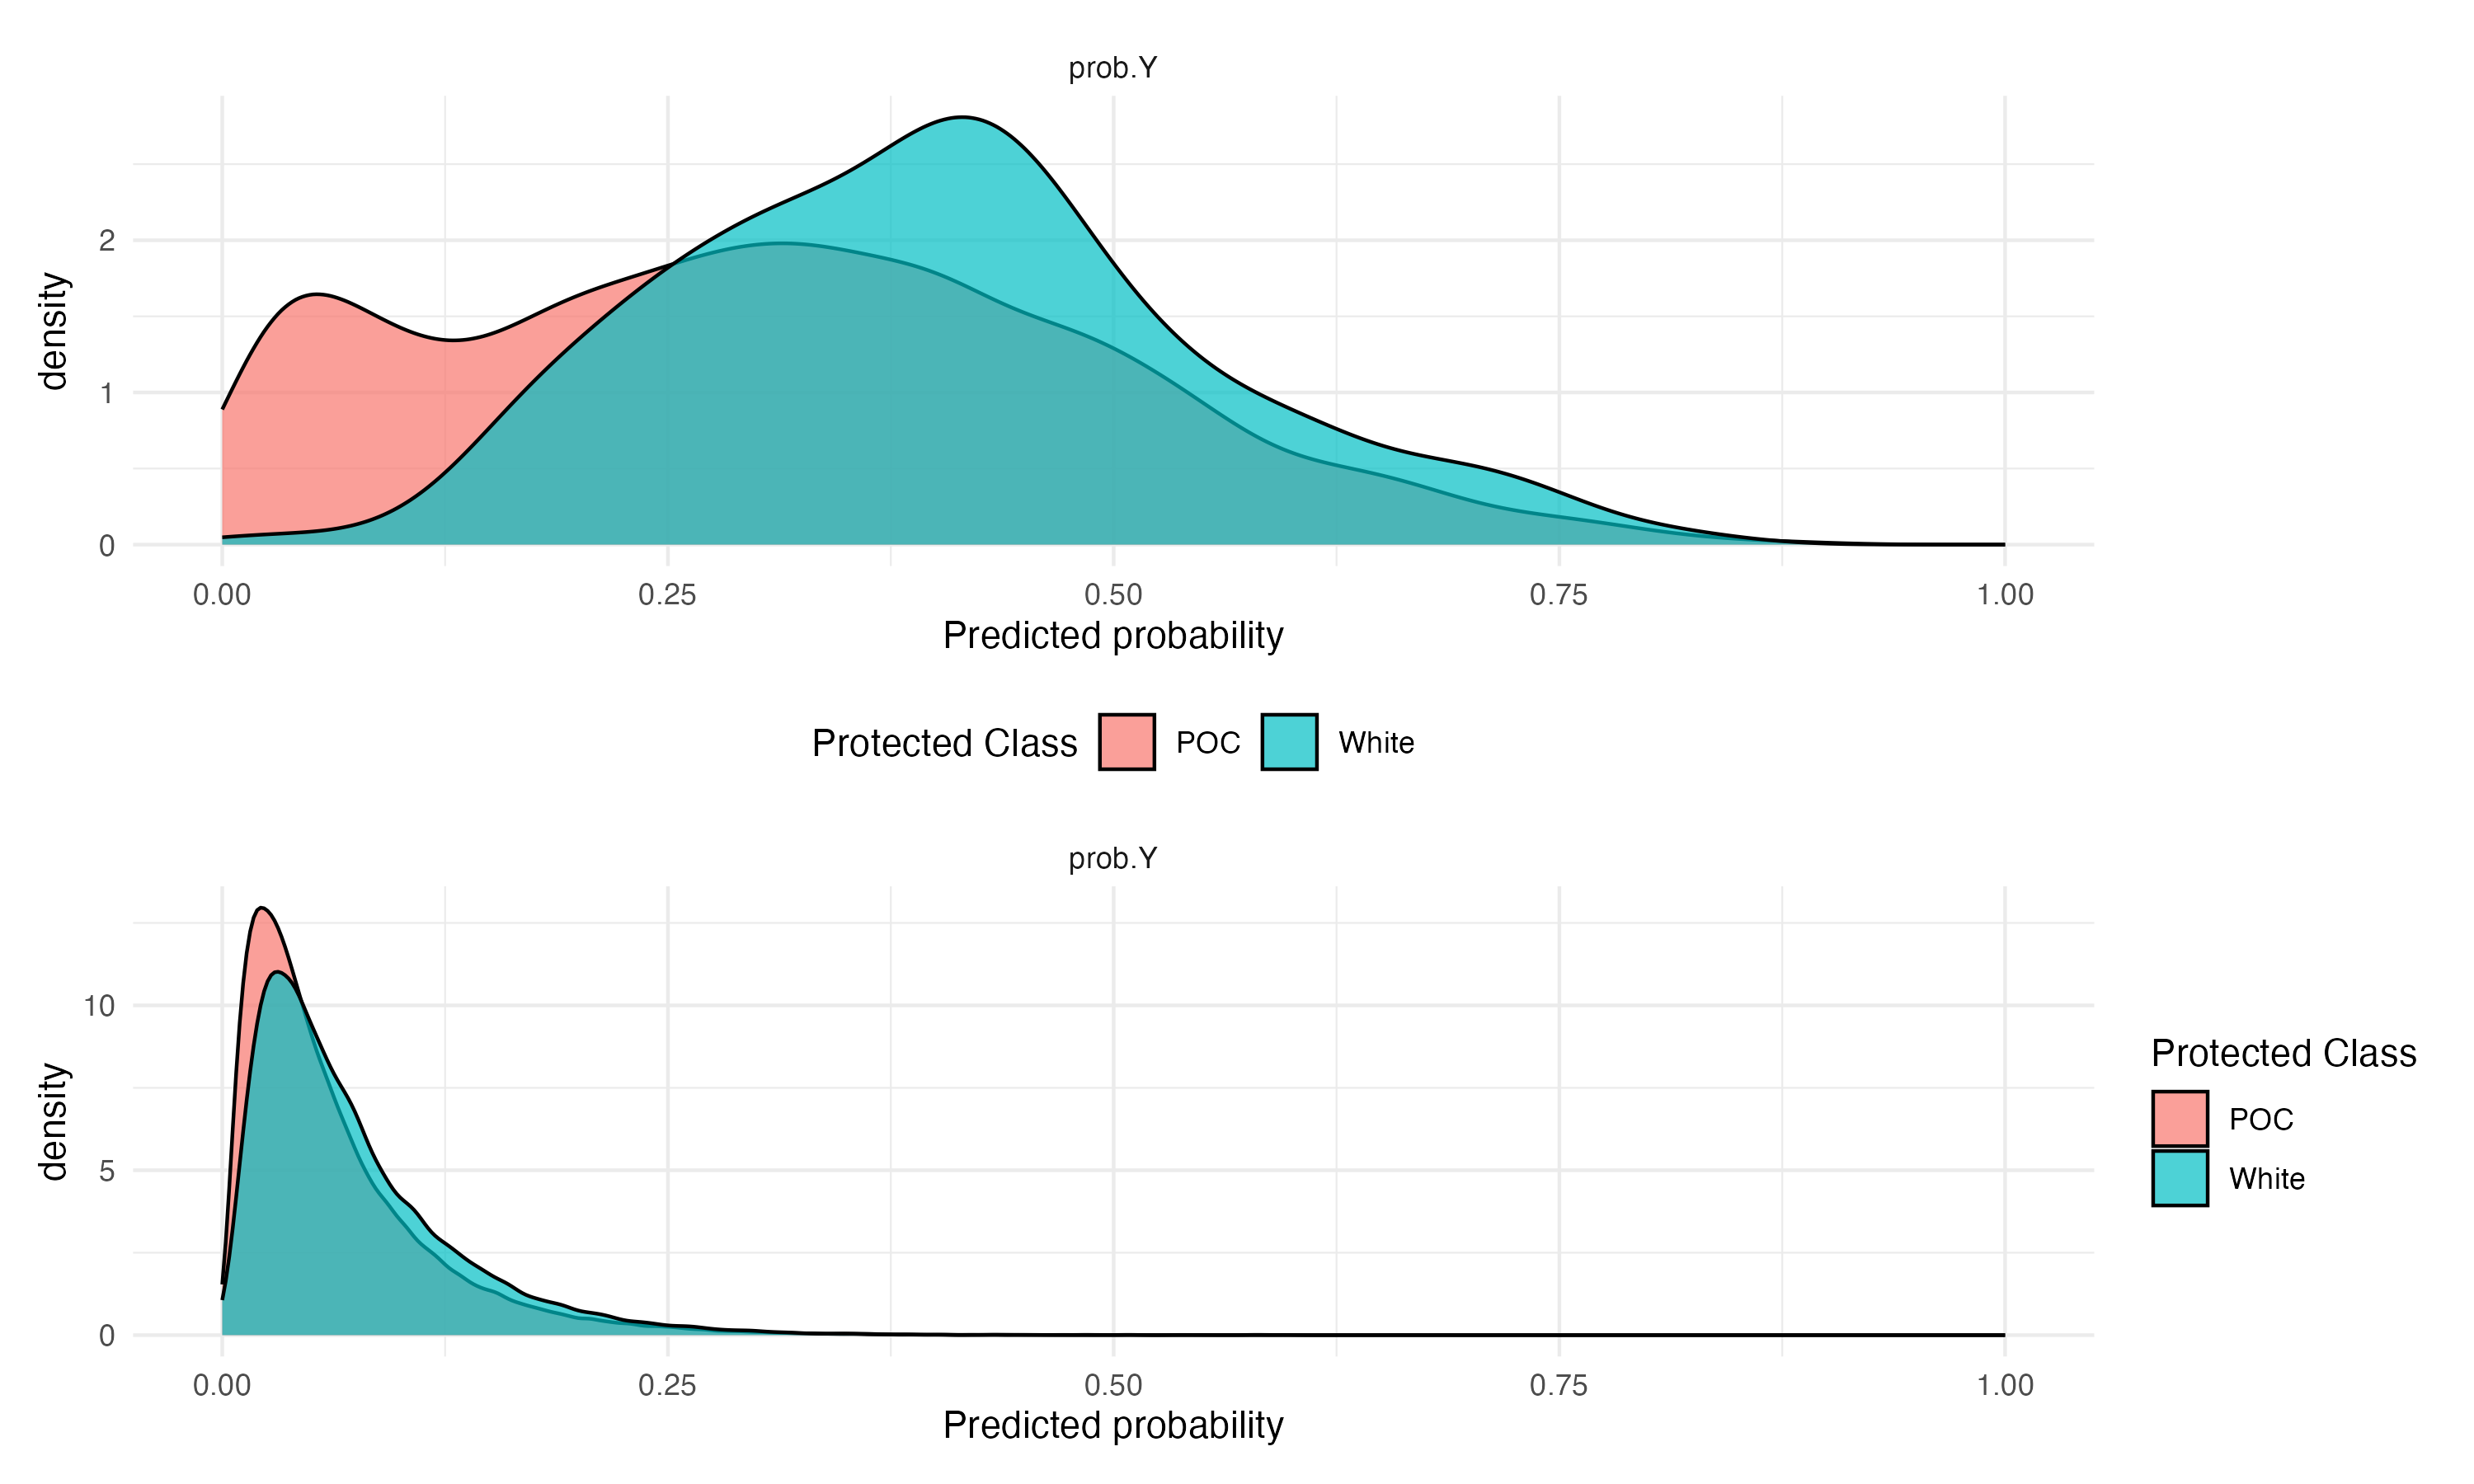
\includegraphics[width=0.7\textwidth]{../figures/sqf_case_study_plot7.png}
    \caption{Density of predicted probabilities both groups.}
    \label{fig:fairness_density}
\end{figure}
To train a random forest classifier on the 2023 data to predict the arrest of a person, we dichotomise the race attribute by grouping "Black" and "Hispanic" as people of colour ("PoC") and "White", "Asian", and "Other" as white ("White").
With many of the group fairness metrics implemented in mlr3fairness, we can measure the (group) fairness of our models.
As suspected after data description, we find that the random forest classifier is already fair. There are minor differences between groups, but exact equality cannot be expected. It is common to allow for a certain margin of error $\epsilon$ in practice.
Especially the error rates (fnr, fpr) are very similar between groups, thus Separation seems to be satisfied overall. Sufficiency metrics have larger differences, though they are still minor. mlr3fairness offers functions to easily visualise fairness. First, in \autoref{fig:fairness_density} we plot the density of risk scores output by the random forest for each group.
The risk score represents the probability of getting a positive prediction $P(\hat{Y} = 1)$, which is undesirable in the SQF context. White subjects tends to have higher predicted probabilities of being arrested, their mode lies around 0.15 while the mode of the PoC group is around 0.05. This means we have more low-risk PoC in the data. Next, from \autoref{fig:fairness_metrics_barplot} we can see that the positive predictive value (Sufficiency) has a relatively large difference between groups,
while the false positive rate is practically the same between groups (Separation). It comes to no surprise that equalised odds, which is based on error rates, is satisfied. Finally, the accuracy between groups is not as equal as the error rates, but the absolute difference is still smaller than 0.05, which is a common $\epsilon$ to choose.
Given that the classifier is fair from a group perspective, it does not make sense to experiment with any of the implemented fairness methods in mlr3. At most, we could try to address the disparities in sufficiency metrics, but the common methods in the package are designed to address concerns with independence or separation. \\
\begin{figure}
    \centering
    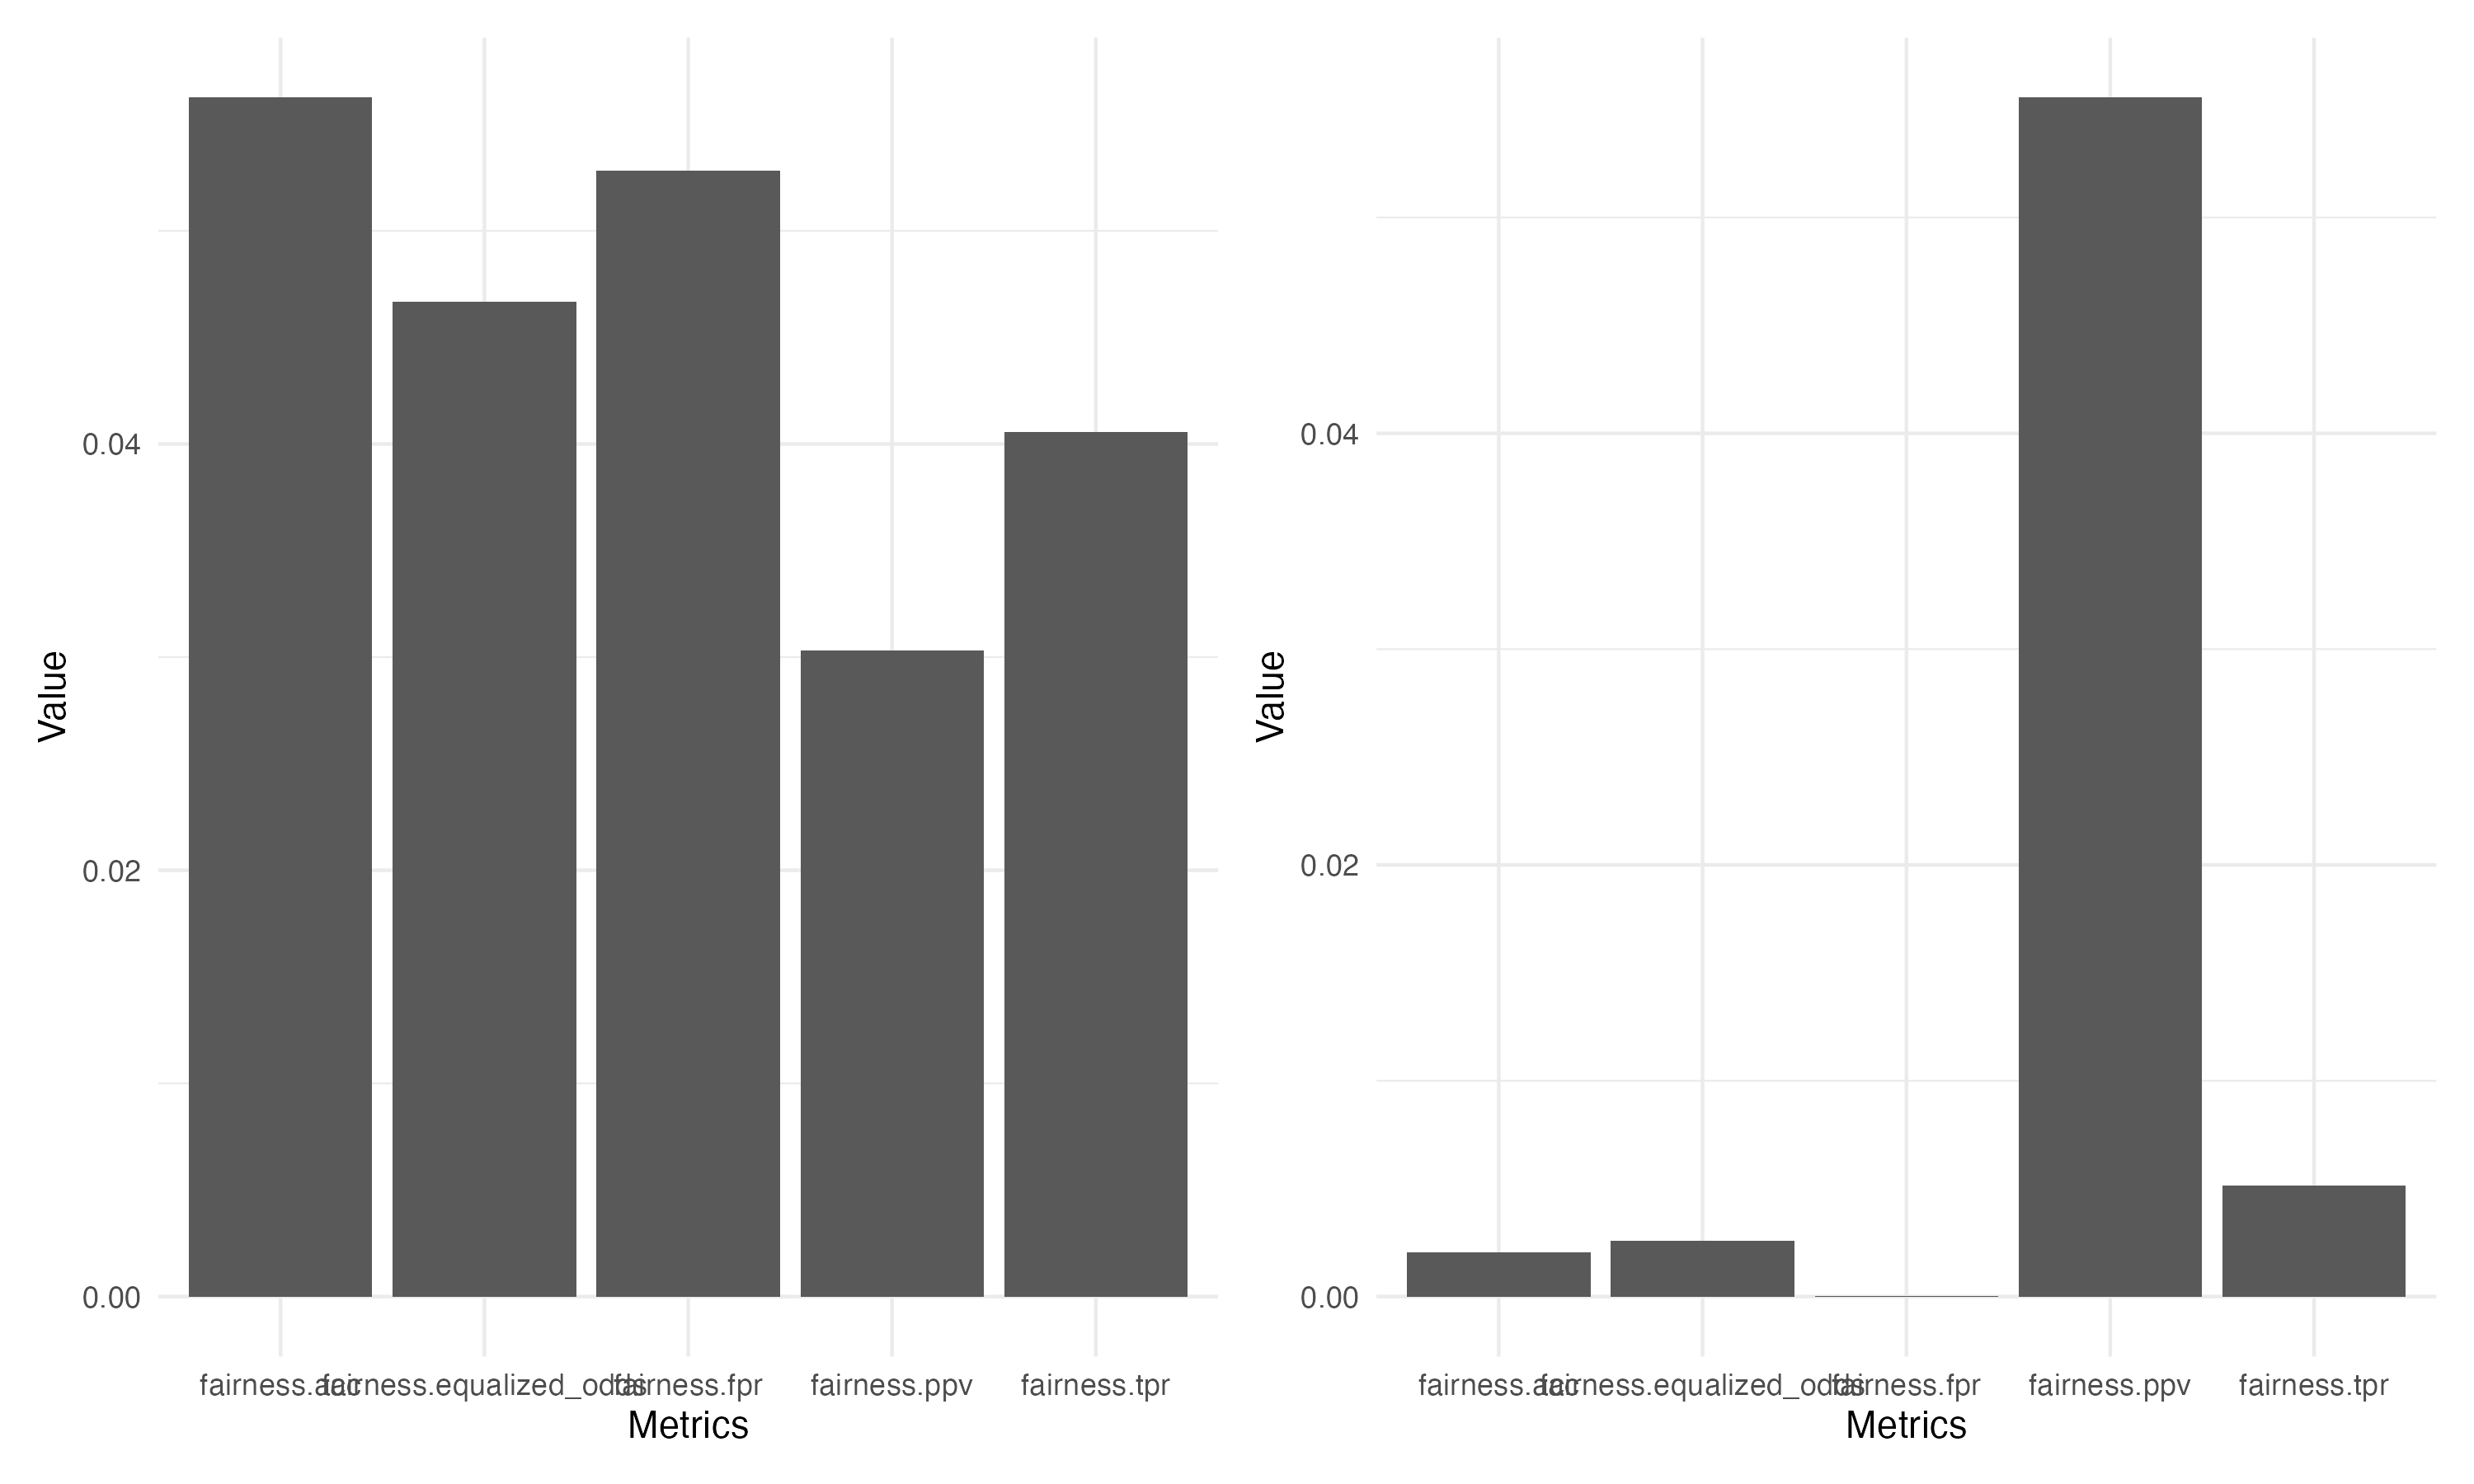
\includegraphics[width=0.7\textwidth]{../figures/sqf_case_study_plot8.png}
    \caption{Comparison of fairness metrics.}
    \label{fig:fairness_metrics_barplot}
\end{figure}

\subsubsection{Fairness Experiment}
Inspired by the chapter on fairness in the mlr3book, we decide to experiment with some fairness methods for the SQF data. \texttt{mlr3fairness} currently has two preprocessing methods, one postprocessing method and several fairness adjusted models implemented. We decide to use a reweighing methods that works with assigning weights to the observations to equalise the distribution of $P(Y|PA)$.
The inprocessing method is a fairness-adjusted logistic regression implemented in \texttt{mlr3fairness} inspired by Zafar et. al. This method optimises for statistical parity (independence). The postprocessing method we choose aims for equalised odds and it works by randomly flipping a subset of predictions with pre-computed probabilities in order to satisfy equalised odds constraints.

It is more interesting to compare the classifier trained on data that comes from the unconstitutional period 2004 to 2012. We decide for 2011 as it is the year with the most stops.
We carry out the same data cleaning steps for the 2011 data as before, starting with 685724 recorded stops and reducing this to 651567 clean observations. Note, these are more than 50 times more stops than in 2023.
The 2011 data has substantially more low-risk stops, only around 6\% of stops result in an arrest. This is a stark contrast to the 2023 data, where 31\% of stops result in an arrest.
The differences in arrestment rates between groups are slightly lower for 2011 and the highest arrestment rate remains to be for the white group. \autoref{fig:arrestment_rates_clean_data}
Due to the large proportion of low-risk stops in 2011 the predicted probabilities are generally low. The x-axis is cutoff at a probability of 0.1, otherwise it would be hard to see anything as the vast majority of probability mass lies in the small regions.
The measured racial disparities are interestingly not greater than in 2023. We see that for the classifier trained on 2011 stops, equalised odds has the greatest difference, but overall the differences in predictions rates across groups are very small. \\ 
Our fairness audit did not show any substantial disparities in fairness metrics. Does this mean the classifier is fair?
It is easy to come to such conclusions, especially if fairness is not the major concern of the practitioners but more of a nuisance criterion that should be fulfilled. However, to truly ensure a fair practice, it is crucial to look at the context in which the algorithm is embedded.

\begin{figure}
    \centering
    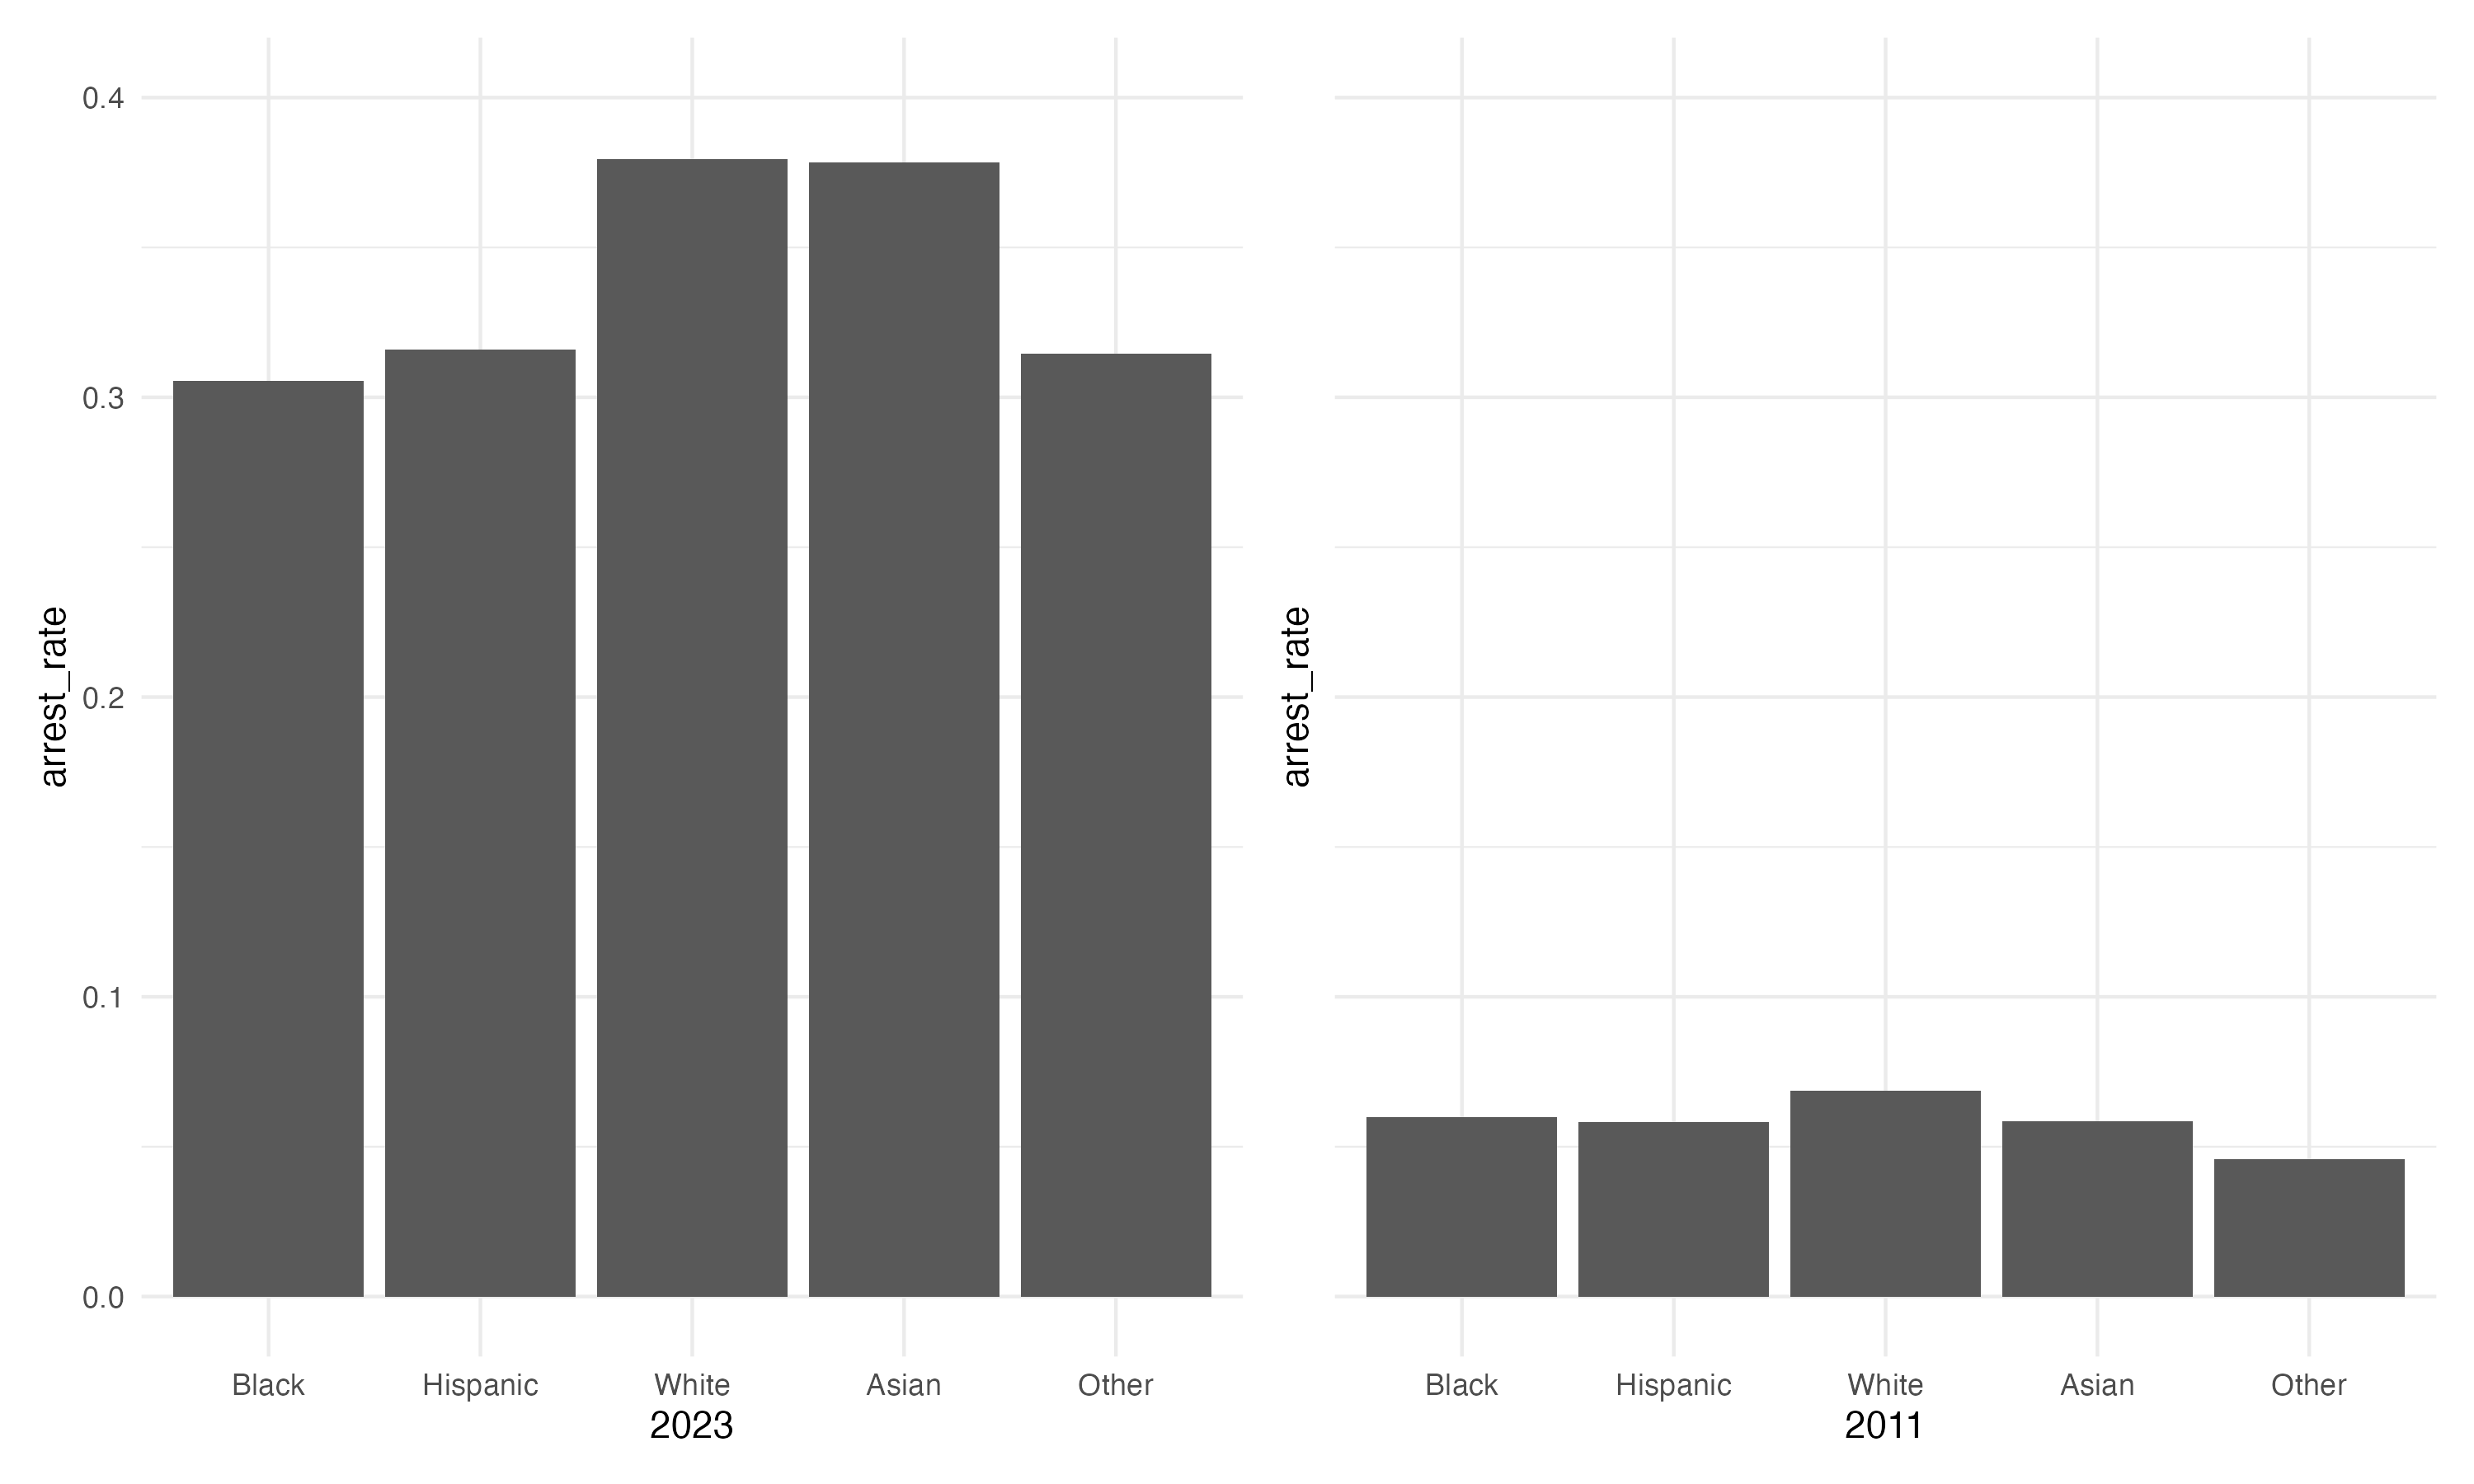
\includegraphics[width=0.7\textwidth]{../figures/sqf_case_study_plot10.png}
    \caption{Comparison of arrestment rates for 2023 (left) and 2011 (right).}
    \label{fig:arrestment_rates_clean_data}
\end{figure}

% \textbf{Fairness Experiment}
% - fairness metrics (table) for dichotomised race and for full race grouping in appendix.
% - fairness methods (inspired by the article)

% Reweighing: https://mlr3fairness.mlr-org.com/reference/mlr_pipeops_reweighing.html?utm_source=chatgpt.com#format
% Fair logistic regression: https://rdrr.io/cran/mlr3fairness/man/mlr_learners_classif.fairzlrm.html?utm_source=chatgpt.com
% EOd: https://mlr3fairness.mlr-org.com/reference/mlr_pipeops_equalized_odds.html?utm_source=chatgpt.com
% mlr3book: https://mlr3book.mlr-org.com/chapters/chapter14/algorithmic_fairness.html?utm_source=chatgpt.com#bias-and-fairness
% https://mlr3fairness.mlr-org.com/#debiasing-methods


% mlr3fairness currently has two preprocessing methods, one postprocessing method and several fairness adjusted models implemented. We decide to use a reweighing methods that works with assigning weights to the observations to equalise the distribution of $P(Y|PA)$.
% The inprocessing method is a fairness-adjusted logistic regression implemented in mlr3fairness inspired by Zafar et. al. This method optimises for statistical parity (independence). The postprocessing method we choose aims for equalised odds and it works by randomly flipping a subset of predictions with pre-computed probabilities in order to satisfy equalised odds constraints.
\subsubsection*{Bias and the feedback loop}
\begin{figure}
    \centering
    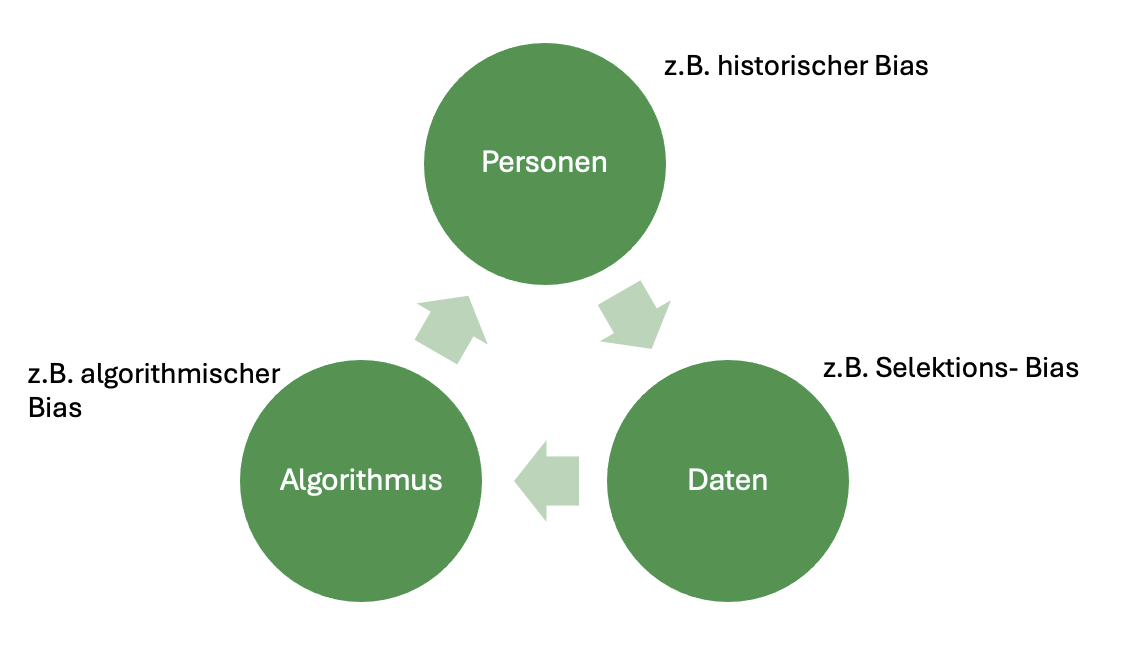
\includegraphics[width=0.7\textwidth]{../figures/bias_loop.png}
    \caption{The bias loop.}
    \label{fig:bias_loop}
\end{figure}

Usually fairness is a concern in the first place, because the algorithm should be implemented as an ADM to assist decision-making in some way. As such it could influence if someone gets admitted to college, gets a loan or is released from prison. The algorithm does not exist in isolation, but is embedded in a loop with data and the user.
We make the circumstances of a decision measurable by collecting data. The algorithm learns from this data to make an optimal prediction, on which the decision-makers base their judgement on ()\autoref{fig:bias_loop}). At each step of this loop, bias can be introduced in the process and, more dangerous, be amplified as the algorithm influences decision-making on a large scale.
This means that every fairness project comes with the task to understand where the data comes from and how exactly the algorithm will be deployed in practice. Let us therefore take a step back and look at the context of the SQF data.

% The data introduced three main challenges: selection bias; missing data; class imbalance.



% borough specific graphics?

% - number of stops conducted but with background information who governed at that time (see Obsidian)
% - transparent explanation of feature selection (similar to Data Transparanecy paper)
% - distribution of race in SQF data vs NYC
% - grouping to black, white, black hispanic, white hispanic, others --> arrestment rates in these groups



\section*{Residual Unfairness}
The main message of this paper is that it is not that easy to adjust for fairness, when the data the algorithm learns from is biased. Ensuring Equal Opportunity or Equalized Odds on the training data does not generalize to the target population. The paper proposes a way to estimate the TRP and FPR in the target population. This is useful, when the fairness methods depends on the FPR and/or TPR. 

This translates as follows to SQF. The police officer decides to stop an individual and this decision might be based on prejudice against certain groups. Further information, such as the possesion of a weapon or the arrestment of a person, is naturally only made on people who were stopped.
This means our training data does not represent the population we want to use the algorithm on, i.e. the stopped individuals are not representative for the population of NYC at a whole. $rightarrow$ compare race distributions or borough distributions (or both)

\cite{kallus} defines fairness via equal opportunity or equalised odds. They argue that even after fairness adjustments on the training population, such as thresholding, discrimination in the target population will remain.
Thus they design a way to estimate the true positive rate and false positive rate of the target population based on training data. A method that uses the TPR and FPR of the data (such as the method proposed by \cite{hardt2016}) can use these adjusted estimations instead and like this ensure fairness on the target population.



Residual Unfairness \cite{kallus} concepts defined in the paper:
Disparate benefit of the doubt: one group gets an advantage over the other by historically repeated better treatment of the group
Equal opportunity and Equalised odds --> from this they define "Inequity of Opportunity" to quantify fairness
First-order stochastic dominance (Def. 3): one group has consistently higher probability scores than the other
Strong disparate benefit of the doubt; Strong disparate benefit of the doubt,  strict;
Weak disparate benefit of the doubt, strict; Weak disparate benefit of the doubt on disparately endowed groups

Currently I understand it as follows:
The different disparate benfits of the doubt fromalise different historical treatment of groupds.
We distinguish two groups in our population, a (advantaged) and b (disadvantaged). Within each group a and b we further dinstiguish between training population (Z=1) and target population (T=1).
My current understanding for Preposition 2: Some propositions now illustrate the scenario, in which repreated deiscriminatory treatment looks like this: For group a the scores in the training population are strictly lower than the scores in the target population. For group b the scores in the training population are strictly higher than in the atrget population. The consequence is that the classifier learn on average low scores for group a, resulting in lenient treatment of group a (which is beneficial in this scenario, $\hat{Y} = 1$ is desired). For group b the opposite mechanism occures, resulting in stricter treatment of group b.
My current understanding for proposition 3: When we design a classifier that that satisfies equal opportunity as fairness criterion under the situation described by preposition 2, then the classifier will not satisfy their definition of fainress/ will show Inequity of opportunity

Preposition 2:
For group a the scores of the target population are always strictly higher than
of the training population. This means that we will learn a comparatevily low threshold for group a.
When we employ the algorithm in the target population, group a member will receive the positive outcome
 more easily (receive benefit of the doubt) because the thresholds is so low. For gorup b
 the opposite is true. The scores in the training data are really high compared to the overall population.
 This means we learn a high threshold for group b. When the system is applied on the whole population it will
 be harder for a random person from group b to receive the advantage because their threshold is so high.
Applied on the SQF data this could translate as follows. First of all, the interpretation shifts. $\hat{Y} = 1$ is 
no longer desirable and we can interpreate scores as riskscores $G_g^{E}$. This means a high thresholds for being classified as $\hat{Y} = 1$ is desirable, a low
threshold is undesirable. We assume that officers were more lenient to stop black individuals, which means that the scores (probability of actually having committed crime) in the training population
of black people are lower than the scores of the target population of black people.
$G_b^{Z=1} \preceq G_b^{T=1}$. This means we will learn a lower threshold for black people(???) \footnote{Why do we learn a lower threshold for black people. Maybe something like this happens: So when a group is super leniently stopped we will have many truly innocent and few truly guilty.}
When we apply the algorithm to the target populaiton we will be more likely to classify black people as $\hat{Y} = 1$ because the threshold is so low. White people, on the other hand,
were selected more strictly. This means that the scores of white people in the training population are higher than the scores of white people in the target population.
$G_w^{Z=1} \succeq G_w^{T=1}$. This means we will learn a high threshold for white people. When we apply the algorithm to the target population we will be less likely to classify white
people as $\hat{Y} = 1$ because the threshold is so high. -- Still unsure if this makes sense, if a transfered it correctly.

For the other group we have many truly guilty and less truly innocent. When now 80\% of truly guilty are classified as guilty in the advantaged group then we would want want 80\% of
the truly guilty to be correctly labelled as guilty in the disadvantaged group. This would only results in lowering the threshold for the disadvantaged group
(so making it easier to predict them as guilty) if we predicted low risk scores for truly guilty people in the disadvantaged group
 Because for equal opportunity we are only looking at the people who were really guilty. So we are basically saying that the large proportion of truly
 innocent people in our sample of the disadvantaged leads to lower risk scores even in the truly guilty group of the disadvantaged (like a spill over effect).
 Only then it would make sense to say that a fairness intervention would compensate by setting lower thresholds for the disadvantaged group. Is this happening? 

Chapter 6: Case study on SQF data
Their main message is always, bias in, bias out. fairness interventions, done on the trainign data are not enough, if your sample is biased, your model will be biased (even after fairness interventions).
They show this in the following way. The goal is to predict innocence of an individual. Such an ADM could help officers
decide who to stop in the first place. The SQF data serves as training data and is naturally censored. The censoring process is that we only
observe innocence of a person if they were stopped. But the decision to stop someone could be based on a biased decision policy.
So we have our censored training data (SQF data). We know that this training data is not representative of the population of NYC in general defined via
location specific variables. Kallus and Zhou use train a logistic regression classifier on the SQF data as is and use post-processing proposed
by Hardt et al. to ensure Equal Opportunity or Equalized Odds. They use their a weighing technique (proposed by them and inspired by propensity score matching)
to simulate the target population. The fairness intervention in the training population produces group-specific thresholds that are then applied to the target population.
They use these fairness-adjusted threshold for the target population and still observe unfairness.

But of course they observe unfairness because the fairness intervention they do is a post-processing step and doesn't modifiy the classifier. What am i not getting here?
\section*{Bias in, bias out - an alternative perspective}

% mathematical definitions I really need to get the point across
% - population as tupel of random variables (X, U, A, Y)
% - taste-based discriminator https://link.springer.com/referenceworkentry/10.1007/978-981-33-4016-9_1-1

An interesting perspective on this observation can be found in \cite{RambachanBBOEFW}. They take a different stance on the problem of biased training data than \cite{kallus} and question the "bias in, bias out" mechanism.

They formalise the problem as follows. For the decision-maker (the police) an individual is characterised by the random vector $(X, U, A)$, where X and A have the same meaning as in \cite{kallus}
and U is a set of unobserved features. These latent variables are unknown to the algorithm but are characteristics the police bases their decision to stop someone on. In the SQF context this could be the personal impression the officer got of a suspect which is not recorded and hard to measure.

The paper assumes the police is a taste-based classifier against African-Americans. This means they hold some form of prejudice against the group of African-Americans that influences their decision to stop a member of this group.
In general, for stopping any person, an officer incurs a cost c > 0. If they stop an individual that turns out to be involved in criminal activity and is therefore arrested, the officer receives a reward b = 1 \footnote{The reward can set to any number b > 0. We assume b = 1 as in \cite{RambachanBBOEFW} without loss of generality.}. In case of stopping an innocent person b = 0.
For stopping African Americans the payoff an officer expects increases by $\tau > 0$ compared to stopping a white person. The total payoff for stopping an individual is given by:
$$Y + \tau * A - c$$
where $Y$ is the outcome of the stop, $\tau$ is the discrimination parameter, $A \in \{0,1\}$, and $c > 0$ is the cost for stopping a person.
Holding the costs $c$ and the outcome of the stop $Y$ constant, searching an African American results in a higher payoff than searching a white person. The goal of the police is to maximise their payoff. Therefore they stop an individual according to the following threshold rule:
$$Z(X, U, R) = 1(E[Y|X, U, A] \ge c - \tau * A)$$
This means that the threshold for stopping an African American is \textit{lower} than for stopping a white person. Consequently, the police stops African Americans more leniently than white people.
This taste-based discrimination rule is the biased decision policy introduced in \cite{kallus}. In \cite{RambachanBBOEFW} the authors speak of "selective labels" where again the tupel $(Y, X, A, Z)$ is only available for $Z = 1$. 

In short: It actually depends on the outcome and the training sample whether the discrminiation of the previously discriminated (bias interhitance) exists. In some cases it can actuall come to the opposite effect, which they call bias reversal.
The mechanism is as follows: the historically discriminated groups is very represented in the sample as being included is an act of discrimination itself. This means we have more training data for the disadvantaged group, they resemble the target population more, as they were more leniently included, and thus the classifier generalised better to the disadvanteged group.
When we collect more data for the group, we come closer to the target population and our classifier will work better on the target population for the group with more data.


Black people are more leniently stopped, leading to higher stopping rates in for black people in the training data, meaning
more training data for this group. Because we stop black peopel more leniently, we record many innocent black people in our data.
In \cite{kallus} this would lead to a lower learned threshold \footnote{first this leads to lower risk scores for black individuals. And then via fairness adjustments (e.g. for equalized odds) this leads to lower thresholds for black individuals.}
for black individuals. Applied on the target population this would mean that we would predict too many false positive. The threshold estimated from the training 
data is so low that we classify to many people as guilty because in the target populations the scores are actually higher and meet the threshold easily.
In \cite{RambachanBBOEFW} they say that by stopping (searching, they actually talk about searching, not stopping) black people so leniently, our sample for black people comes actually pretty
close to the target population.
In other words, the training data for black people is pretty close to the target data for black people, which means that our classifier will work well on the
target population for black people. \\
To summarise, in \cite{kallus} bias against a group results in a less representative sample. In \cite{RambachanBBOEFW} bias against a group results in a more representative sample.


\textbf{Theorem 1}\\
The prediction for african americans is weakly decreasing in tau. This means, as tau increases (so racial bias increases), the expected value for Y gets actually lower,
so closer to zero, so less often predicted to have a contraband. What is happening? Higher tau means lower searching threshold for african americans.
So the data for african americans becomes "more noisy", more and more innocent people come into our sample, so we predict lower risk for african americans. 
In \cite{RambachanBBOEFW} paper this translates to a more representative training data for african americans and thus also better performance on the general population of african americans.
In \cite{kallus} paper the mechanisms is the same, we also estimate lower risks cores for african americans, but then sth else happens.
I think in Kallus we then do a fairness intervention that leads us to setting a LOWER threshold for african americans, meaning we predict them as
guilty more easily to achieve the same FPR as in the other group. I think in kallus they first formulate it in the strict way, where the police is so biased against african americans
that the stopped african americans are LESS likely to actually have a weapon than the general population. But they relax this setting afterwards.


What happens if we train the logistic classifier (to predict weapon yes no) on the SQF as is (Kallus), don’t do a post processing fairness intervention (NO Hardt et. al)
and test the classifier on the target population (that is created via the weighing method of Kallus and Zhou)? I think according to \cite{RambachanBBOEFW} we should observe bias reversal.
\newpage

% \includeonly{chapters/introduction.tex, chapters/results.tex}
% include{}

% \section{Data}
% \label{Data}
% \input{Chapter/Data.tex}
% \newpage
\newpage

% ------------------------------------------------------------------------------
% listoffigures ----------------------------------------------------------------
% ------------------------------------------------------------------------------

% \setcounter{page}{3} % CHANGE

\listoffigures
% \input{Chapter/List of figures.tex}

\newpage

% ------------------------------------------------------------------------------
% listoftables -----------------------------------------------------------------
% ------------------------------------------------------------------------------

\listoftables
% \input{Chapter/List of tables.tex}

\newpage

\newpage
\section*{Acknowledgement}

\newpage

% ------------------------------------------------------------------------------
% APPENDIX ---------------------------------------------------------------------
% ------------------------------------------------------------------------------
    
\pagenumbering{Roman}

\setcounter{page}{5} % CHANGE

\appendix

% \section{Appendix}
% \label{app}
% \input{Chapter/Appendix A.tex}
% \newpage

\section{Electronic Appendix}
\label{el_app}


Data, code and illustrations are available in electronic form. \bigskip

% \input{Chapter/Appendix B.tex}
% \newpage

% ------------------------------------------------------------------------------
% BIBLIOGRAPHY -----------------------------------------------------------------
% ------------------------------------------------------------------------------

\RaggedRight
% \bibliography{../literature.bib}
% \bibliographystyle{dcu}
\printbibliography
\newpage
% ------------------------------------------------------------------------------
% DECLARATION OF AUTHORSHIP-----------------------------------------------------
% ------------------------------------------------------------------------------
\Large
\noindent
\textbf{Declaration of authorship} 
\vspace{0.5cm}
\noindent
\normalsize

I hereby declare that the report submitted is my own unaided work. All direct 
or indirect sources used are acknowledged as references. I am aware that the 
Thesis in digital form can be examined for the use of unauthorized aid and in 
order to determine whether the report as a whole or parts incorporated in it may 
be deemed as plagiarism. For the comparison of my work with existing sources I 
agree that it shall be entered in a database where it shall also remain after 
examination, to enable comparison with future Theses submitted. Further rights 
of reproduction and usage, however, are not granted here. This paper was not 
previously presented to another examination board and has not been published.
\\

\vspace{1cm}
\textcolor{orange}{Munich, \mydate} \\

\vspace{3cm}

\noindent\rule{0.5\textwidth}{0.4pt} \\

\textcolor{orange}{\myname}

\end{document}
